\chapter{Image Processing}
\label{chap:image_processing}

\begin{figure}[ht]
	\hfill
	\begin{minipage}{0.5\textwidth}
		\centering
		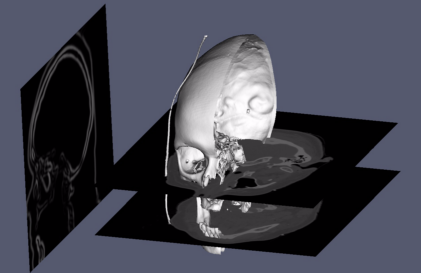
\includegraphics{VTKTextbook-216}
		\caption*{\texttt{Gradient magnitude of a slice (vertical) of the Visible Woman CT dataset shown with an isosurface and two slices (horizontal) of the dataset.}}
	\end{minipage}
\end{figure}

\firstletter{I}n this chapter we describe the image processing components of the Visualization Toolkit.
The focus is on key representational ideas, pipeline issues such as data streaming, and useful algorithms for improving the appearance and effectiveness of image data visualizations.

\section{Introduction}

Image processing has been a mainstay of computing since the advent of the digital computer. Early efforts focused on improving image content for human interpretation. More recently image processing has been utilized by practitioners of computer vision, the goal being the processing of image data for autonomous machine perception \cite{Gonzalez92}. From the perspective of data visualization, image processing is used to manipulate image content to improve the results of subsequent processing and interpretation. For example, a CT or MRI scan may generate spurious signal noise or require image segmentation. Using the techniques of image processing, noise can be removed and automatic and semi-automatic segmentation can be performed on a slice by slice (i.e., image by image basis). As a result, isosurface generation, volume rendering, and other 3D techniques can be improved in appearance, accuracy, and effectiveness by applying techniques from image processing.

Since the focus of this text is on 3D graphics and visualization, this chapter treats image processing in a limited way. However, we would like to emphasize the interrelationship of image processing, computer graphics, and visualization. Often texts and courses treat these as distinctly separate disciplines, when in fact they are closely related (see ``Imaging, Computer Graphics, and Visualization''on page \pageref{sec:imaging_computer_graphics_visualization}).

The material presented here was selected to demonstrate a number of important points. First, the data flow or pipeline approach presented earlier is directly applicable to image processing, with the added benefit that we can easily implement data streaming and caching due to the regular nature of image data. Second, image processing algorithms can improve the results of visualization. We will show this through a number of useful examples. And finally, from a practical point of view, we wanted to demonstrate a system architecture that includes imaging, graphics, and visualization.

\section{Data Representation}

In this section we will briefly describe the data representation behind the imaging pipeline. As we saw earlier (in ``The Dataset'' on page \pageref{sec:dataset}), a dataset consists of both a structure (topology and geometry) and data attributes. Although in principle an image can be represented as a image data dataset, the special nature of image processing suggests a more complex representation, as we will soon see.

An image is typically used to refer to a 2D structured point dataset. More generally, in this chapter we will define an image as consisting of up to four dimensions: three spatial dimensions x, y, and z, and time t. The reason we add the time dimension is that images are frequently generated as a time series, and we often wish to access the data along the time axis. For example, we may plot the value at a point as a function of time.

As described in ``Image Data'' on \pageref{subsec:image_data}), an image has both regular topology and geometry. The regularity of the data lends itself to many special operations. In particular, we can support data caching and \emph{streaming}, and operating on \emph{regions of interest} in the data.

\subsection{Regions of Interest}

When data has a regular spatial organization, it is possible to request the data in pieces or regions of interest. For example, a mapper may need only a region of the data for its display, so loading or processing the whole dataset would be inefficient. An example of this is a two-dimensional viewer that displays only one slice of a large structured volume. By loading slices only as they are needed, disk access can be reduced, and memory conserved.

\begin{figure}[htb]
	\begin{subfigure}[h]{0.36\linewidth}
		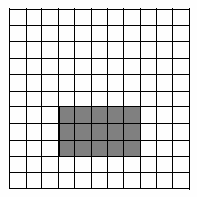
\includegraphics[width=0.96\linewidth]{Figure10-1a}
		\captionsetup{justification=centering}
		\caption*{Axis aligned matrix (rectangular region)}
		\label{fig:Figure10-1a}
	\end{subfigure}
	\hfill
	\begin{subfigure}[h]{0.36\linewidth}
    % Dummy spacer
	\end{subfigure}
	\hfill
	\begin{subfigure}[h]{0.36\linewidth}
		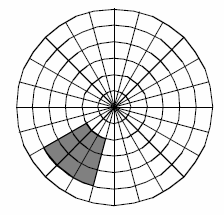
\includegraphics[width=0.96\linewidth]{Figure10-1b}
		\captionsetup{justification=centering}
		\caption*{Polar coordinate grid (pie shaped region)}
		\label{fig:Figure10-1b}
	\end{subfigure}
	\caption{Axis aligned matrices naturally lend themselves to rectangular regions, and polar coordinate grids to pie-shaped regions.}\label{fig:Figure10-1}
\end{figure}

Although regions of interest can have arbitrary shapes, the regular structure of the data samples determines optimal region configurations. An image stored in a Cartesian coordinate system easily divides into smaller rectangular regions, while data sampled on a polar coordinate grid is best divided into pie-shaped regions (Figure \ref{fig:Figure10-1}). Therefore, operating on regions of data means that we process ``windows'' of data specified by $(min,max)$ ranges of each dimension, or axis. For example, a region in a 2D image of dimensions $100 \times 100$ might be specified as $(25,49, 0,49)$, meaning that we would operate on a $(25 \times 50)$ window.

\subsection{Streaming and Caching}

The disadvantage of processing regions of interest is that the same data may be read and processed multiple times. If the viewer described above needs to cine (i.e., loop) through the slices, or interactively pan around a large image, it would be beneficial to have all the data loaded at once.

A compromise between the two extreme approaches of maintaining all data in memory or operating on small pieces is to update regions larger than requested, but not as large as the whole image. This is referred to as a data cache. Data caching anticipates future requests and works well in most cases. However, it breaks down when there is little or no coherence between subsequent requests.

With the region-processing model, the data objects can be thought of as caches that hold any number of regions. There are numerous caching strategies for saving and releasing regions that can be quite complex. The simplest strategy saves only a single region at any one time. If subsequent requests are completely contained in the cached region, no further processing is required. An alternative strategy might divide an image into tiled regions of all the same size. When a region larger than the tile is requested, multiple tiles are updated to cover the region. When designing a caching strategy, it is important to consider the overhead of copying data to change its format. Some of the advantages of complex strategies are lost when all the factors are considered.

Given the ability to operate on regions of data, it is a small step to \emph{stream} operations on a whole dataset. Streaming is the process of pulling regions of data in a continual flow through the pipeline. For instance, a pixel histogram mapper could request single pixels as it accumulates values in its bins. Large datasets can be processed in this manner without ever having to load more than a few pixels at a time. If multiple processors are available, region processing can also be used to split a task into multiple pieces for load balancing and faster execution.

\subsection{Attribute Data and Components}

Unlike visualization algorithms that may generate normals, vectors, tensors, and texture coordinates, image processing algorithms generally process attribute data consisting of scalar data. Often the data is a single component (e.g., a gray-scale image), but frequently color images (three components of RGB, for example) may also be processed.

In the \emph{Visualization Toolkit} imaging pipeline, attribute data is represented as n-dimensional component data. Refer to ``Putting It All Together'' on page \pageref{sec:chap10.putting_it_all_together}) to see the implementation details for component data, regions of interest, streaming, and caching.

\section{Algorithms}

This section provides an overview and examples for important image processing algorithms. The importance of the algorithms is measured on their relevance to 3D data visualization. Topics include: removing noise, smoothing, reducing sampling artifacts, image enhancement, segmentation, and morphological operators such as erosion and dilation.

\subsection{Image Restoration}

Noise and other artifacts are inherent in all methods of data acquisition. Since artifacts can degrade the visual appearance and analysis of images, the first step of image processing is often restoration. Knowledge of the statistical properties of artifacts allows filters to selectively remove them with minimal impact on the underlying data. For example, most of the power of typical images lie in low frequencies, while white noise is evenly distributed across the frequency spectrum. In this situation, low-pass filters eliminate much of the noise, but leave most of the image intact.

\begin{figure}[htb]
	\begin{subfigure}[h]{0.24\linewidth}
		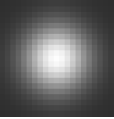
\includegraphics[width=0.96\linewidth]{Figure10-2a}
		\captionsetup{justification=centering}
		\caption*{Gaussian Kernel}
		\label{fig:Figure10-2a}
	\end{subfigure}
	\hfill
	\begin{subfigure}[h]{0.98\linewidth}
		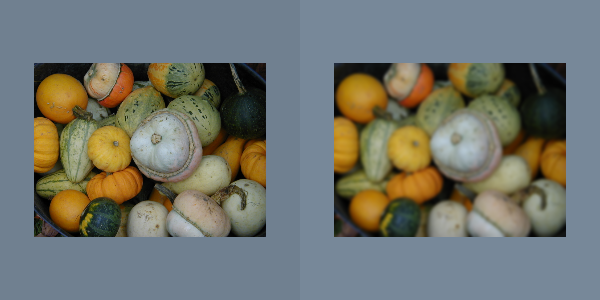
\includegraphics[width=0.96\linewidth]{Figure10-2b}
		\captionsetup{justification=centering}
		\caption*{Original image (left). Convolution (right):
         $f*k(x,y) = \sum_{ij}f(i,j)k((x-i),(y-j))$}
		\label{fig:Figure10-2b}
	\end{subfigure}
	\caption{Low-pass filters can be implemented as convolution with a Gaussian kernel. The Gaussian kernel displayed on top has been magnified for this figure.}\label{fig:Figure10-2}
\end{figure}

A simple implementation of a low-pass smoothing filter is convolution with a kernel with all positive values. The typical kernels used for smoothing are either constant across a circular neighborhood, or have a Gaussian profile (see Figure \ref{fig:Figure10-2}). Gaussian smoothing results in better-looking images than smoothing with constant kernels, but can be more computationally expensive because of the large kernel size necessary to capture the Gaussian profile. Smoothing becomes even more expensive when it is generalized to three-dimensional datasets, and three-dimensional kernels.

One way to speed Gaussian smoothing is to decompose the filter into two 1D convolutions. Since the 2D Gaussian function is separable,

\begin{equation}\label{eq:10.1}
g(i, j) = \dfrac{1}{2\pi \sigma^2} \exp\left(-\dfrac{i^2 + j^2}{2\sigma^2} \right)
        = \dfrac{1}{\sqrt{2\pi}\sigma} \exp\left(-\dfrac{i^2}{2\sigma^2} \right)
          \dfrac{1}{\sqrt{2\pi}\sigma} \exp\left(-\dfrac{j^2}{2\sigma^2} \right)
\end{equation}
\myequations{Decomposing a 2D Gaussian function into two 1D convolutions.}

\noindent smoothing along the \emph{x} axis and then along the \emph{x} axis with 1D Gaussian kernels is equivalent to convolving with a 2D Gaussian kernel. It is also possible to approximate Gaussian smoothing by convolving with a constant binary kernel multiple times.

\subsection{Nonlinear Smoothing}

One problem with simple smoothing to remove noise is that edges are blurred. Although high frequencies make up a small part of images, the human visual system is acutely sensitive to high frequencies in the spatial form of edges. In fact, most of the low frequencies in an image are discarded by the visual system before it even leaves the retina. One approach to smoothing that preserves edges is anisotropic diffusion. This filter smooths relatively flat regions of an image, but does not diffuse across abrupt transitions. The diffusion is iterated until the desired level of noise reduction is reached. Two possible diffusion criteria are: Diffuse only when the gradient magnitude is below a specified value, or diffuse two pixels only when the difference between the pixels is lower than a specified constant.

\begin{figure}[!htb]
	\centering
	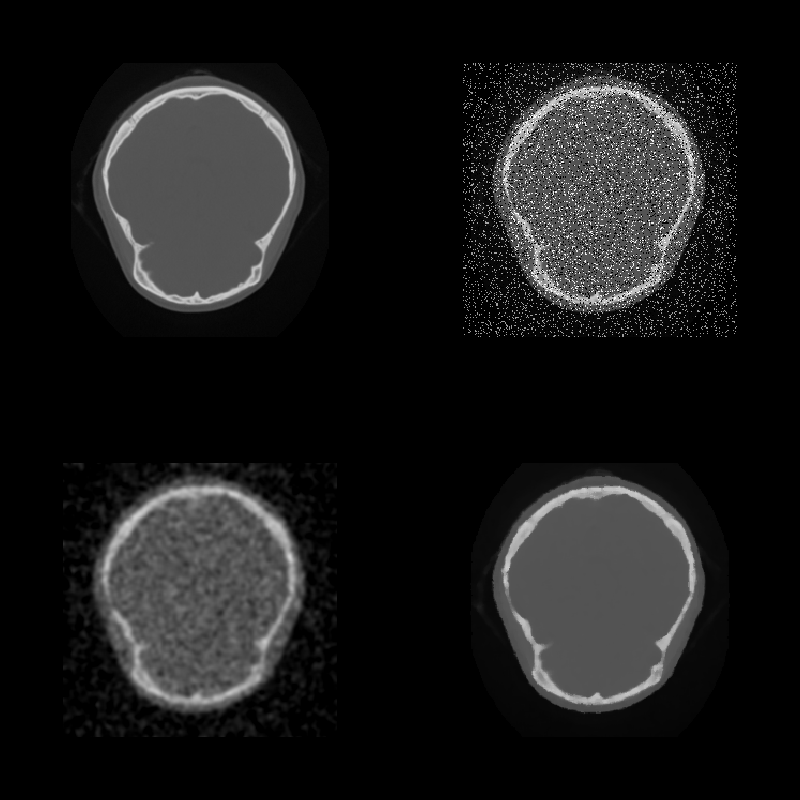
\includegraphics[width=0.98\textwidth]{Figure10-3}
	\caption{Comparison of Gaussian and Median smoothing for reducing low-probability high-amplitude noise. Top row: Original image (left); Noisy image (right). Bottom row: Gaussian smoothing (left); Median smoothing (right).}
	\label{fig:Figure10-3}
\end{figure}

\begin{figure}[htb]
	\begin{subfigure}[h]{0.96\linewidth}
		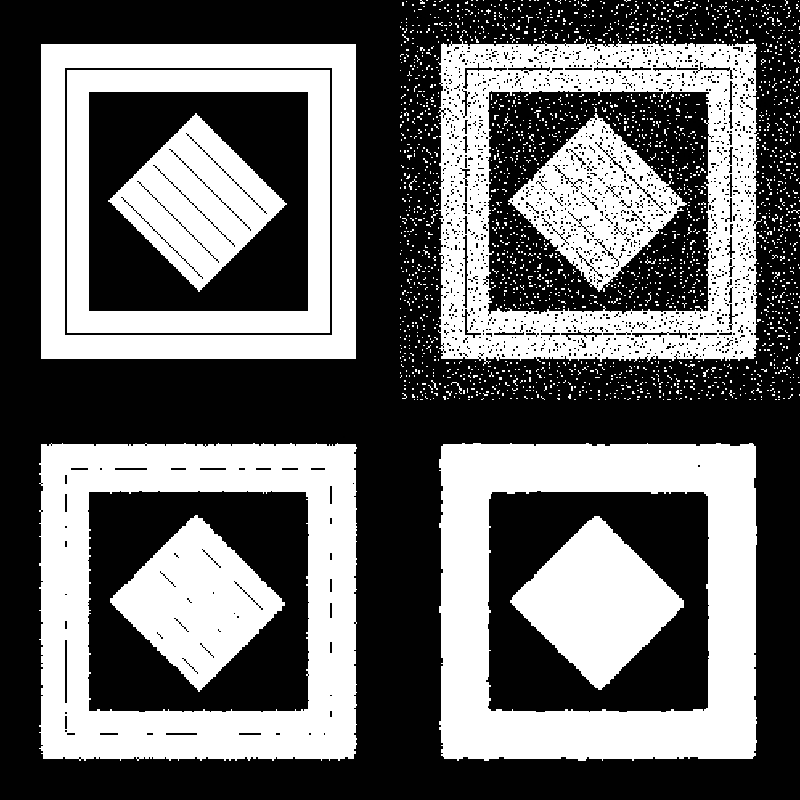
\includegraphics[width=0.96\linewidth]{Figure10-4a}
		\captionsetup{justification=centering}
		\caption*{}
		\label{fig:Figure10-4a}
	\end{subfigure}
	\hfill
	\begin{subfigure}[h]{0.32\linewidth}
		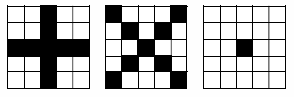
\includegraphics[width=0.96\linewidth]{Figure10-4b}
		\captionsetup{justification=centering}
		\caption*{Hybrid--Median Neighborhoods}
		\label{fig:Figure10-4b}
	\end{subfigure}
	\caption{Comparison of median and hybrid-median filters. The hybrid filter preserves corners and thin lines, better than the median filter. The lower patterns represent the three neighborhoods used to compute the hybrid median. Top row: Original image (left); Noisy image (right). Middle row: Hybrid-median filter (left); Median filter (right).}\label{fig:Figure10-4}
\end{figure}

A median filter also smooths while preserving edges. This filter replaces each pixel with the median value of the scalar values in a neighborhood centered on the pixel. Median filters are most effective on high amplitude noise that has a low probability of occurring (see Figure \ref{fig:Figure10-3}). There are two ways to control the amount and scale of noise removed: The size of the neighborhood can be varied, or the filter can be applied multiple times. This median filter preserves edges; however, it does round corners and remove thin lines. The hybrid median filter was developed to address this behavior. It operates on a $5 \times 5$ neighborhood around each pixel. The algorithm consists of two steps: first the median values of an ``x''-shaped and ``+''-shaped neighborhoods are computed, then the median of these two values and the center-pixel value is computed to give the final result. The hybrid median has a fixed size neighborhood, but can be applied multiple times to further reduce noise (Figure \ref{fig:Figure10-4}).

\subsection{Low Frequency Artifacts}

\section{Putting It All Together}
\label{sec:chap10.putting_it_all_together}

We suggest that you review the code accompanying the images in this chapter to see how to use the VTK imaging pipeline. In this section we will explain some of the implementation details of image data. We will also show how to mix the imaging and visualization pipelines, and how to use imaging filters to perform regression testing.

\section{Chapter Summary}

Image processing can be used to improve 3D visualizations of structured point datasets (images and volumes). Important techniques include smoothing, filtering, morphological operators such as erosion and dilation, and segmentation.

Because of the regular topology and geometry of images, it is possible to design caching and streaming pipelines to reduce memory requirements. In the \emph{Visualization Toolkit}, the imaging pipeline is integrated with the visualization pipeline. This capability enables the creation of applications that combine computer graphics, imaging, and visualization.

\section{Bibliographic Notes}

Many books are available describing imaging algorithms. Several are listed below including \cite{Gonzalez92} and \cite{Russ95}. The texts \cite{Pavlidis82} and \cite{Wolberg90} are imaging books with somewhat of a computer graphics and/or visualization slant. The text \cite{Robb95} is an outstanding reference for medical imaging and visualization.

If image processing, segmentation, and/or registration are important to you, we highly recommend the Insight Segmentation and Registration Toolkit (ITK). Like VTK, ITK is open source and includes extensive documentation resources and examples. Visit \href{https://itk.org/}{ITK} for more information. Also, \cite{Ibanez03} is a good reference.

Technical references describing VTK’s unique streaming visualization pipeline are available \cite{Law99} \cite{Martin01}. Using this approach, data sizes of approximately a petabyte in size have been processed.


\printbibliography

\section{Exercises}

\begin{figure}[!htb]
	\centering
	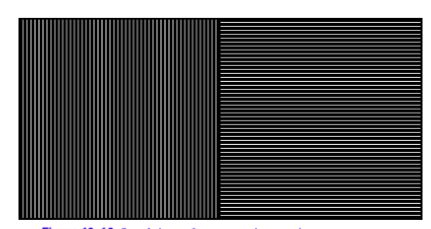
\includegraphics[width=0.98\textwidth]{Figure10-19}
	\caption{Sample image for segmentation exercise.}
	\label{fig:Figure10-19}
\end{figure}

\begin{enumerate}

\item Create an image pipeline that will segment the area with vertical lines in Figure \ref{fig:Figure10-19}.

\item Decomposition can increase the speed of an operation.

    \begin{enumerate}

    \item Prove that 3D Gaussian smoothing can be decomposed into three 1D operations.

    \item Determine the complexity of the decomposed filter and the same filter implemented as a 3D convolution.

    \item Under what conditions can constant smoothing be decomposed into 1D operations?

    \end{enumerate}

\item Create an image pipeline that shows the spectrum of a Gaussian image. What effect does increasing or decreasing the standard deviation have on the spectrum?

\end{enumerate}
